\subsection{Nyquist-Shannon Sampling Theorem}

When recording audio signals, one has to set a sampling rate
(rate for analog signal, frequency for discrete signal). There
are several reasons why we set a sampling rate:

\begin{enumerate}
	\item Data storage conservation,
	\item Bandwidth conservation,
	\item Power conservation.
\end{enumerate}

The formula for sampling is:

\begin{equation}
	x[n]=x(t)|_{t=nT_{S}}=x(nT_{S})
	\label{eqn:signal}
\end{equation}

Where \(T_{S}\) is the sampling period and \(f_{S}=
\dfrac{1}{T_{S}}\) is the sampling frequency 
\cite{notes:class}. Lastly, $n$ is an index of the samples.

However, we have to be careful not to set this sampling rate too
low, or else we run into a problem called aliasing. Low-frequency
aliasing is caused by undersampling, and occurs when a different
time function with a lower frequency produces the same set of
samples \cite{aliase:wiki}. For example, the signal produced by
the function:

\begin{equation}
	x[t]=cos(2\pi10t)
\end{equation}

can be visualized (in the time domain) as:

\begin{figure}[H]
	\centering
	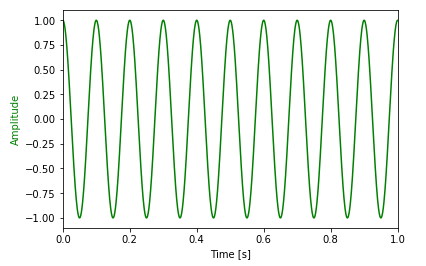
\includegraphics[scale = 1]{images/original_signal.png} %this is useful too \includegraphics[width = \linewidth]
	\caption{Original signal, from equation \ref{eqn:signal} \cite{notebook:sampling}.}
	\label{fig:signal_og}
\end{figure}    

Converting to a discrete signal, by undersampling at 18 Hz rate, we
produce the aliasing, as can be seen below.

\begin{equation}
	x[n]=\cos(\frac{2\pi \cdot 10n}{18})
\end{equation}

Because the signal is periodic, adding or subtracting $2\pi n$ 
inside of the cos function does not change the equation.

\begin{equation}
	x[n]=\cos(\frac{10\pi \cdot n}{9} - 2\pi n)
\end{equation}
\begin{equation}
	x[n]=\cos(\frac{10\pi \cdot n}{9} - \frac{18\pi n}{9})
\end{equation}
\begin{equation}
	x[n]=\cos(-\frac{8\pi\cdot n}{9})
\end{equation}
\begin{equation}
	x[n]=\cos(\frac{8\pi\cdot n}{9})
\end{equation}

By undersampling, we create an alias signal corresponding to
\(8\pi\dfrac{n}{9}\). Our sample rate of 18 Hz is too low. Below
is our sampling overlaid on the original curve.

\begin{figure}[H]
	\centering
	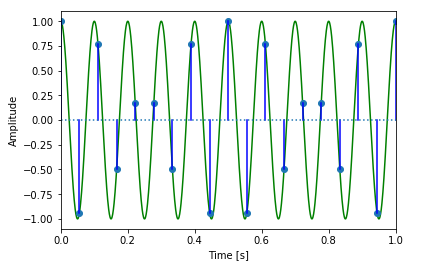
\includegraphics[scale = 1]{images/sub_sample.png} %this is useful too \includegraphics[width = \linewidth]
	\caption{
		Overlaid sampling (in blue) on the original curve (in green) 
		\ref{eqn:signal} 
		\cite{notebook:sampling}.
	}
	\label{fig:sub_sample}
\end{figure}    

This shows that that there are additional functions that can cross
through the sampling points of our original signal, creating
alternative interpretations. For example, in the graph below,
notice that the red curve matching the aliased result is a valid
interpretation of the sampled points originally derived from the
green curve.

\begin{figure}[H]
	\centering
	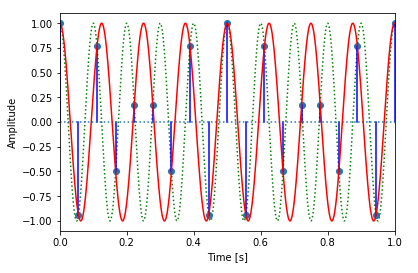
\includegraphics[scale = 1]{images/aliased_curve.png} %this is useful too \includegraphics[width = \linewidth]
	
 \caption{
	The aliased signal (in red) intersects the original
 	signal (in green) at the sampling points (in blue)
	\ref{eqn:signal} \cite{notebook:sampling}.
	} 
 	\label{fig:aliase}  
 \end{figure}

So, if our objective is to sample as little as possible, how do
we determine the minimum rate necessary? The Nyquist-Shannon theorem states that if a function $x ( t )$ contains no
frequencies higher than $B$ hertz, then it is completely determined by
giving its ordinates at a series of points spaced $1 / ( 2 B )$
seconds apart \cite{shannon:wiki}. It then follows that a sufficient sampling rate (nyquist rate) is therefore twice the maximum frequency $B$ Hz, $2B$ \cite{shannon:wiki}.
Restated from a different angle: for a given sample rate $f_{s}$, perfect reconstruction of a signal is guaranteed for a bandlimit $B<f_{s}/2$ \cite{shannon:wiki}.


In our case, before processing with a filter, our raw signal had
a sampling rate of 44.1 kHz. This is the standard for CD-quality
audio. Since human hearing range is roughly 20 Hz to 20,000 Hz, the sampling rate has to at least be 40 kHz (from the Nyquist-Shannon theorem). Audio signals still have to be passed through a low-pass anti-aliasing filter, because even though humans cannot hear frequencies beyond that, these signals can still cause aliasing. A transition band of 4,100 Hz is added to the 40 kHz allows greater ease of anti-aliasing filtering \cite{cd:wiki}. Figure \ref{fig:lowpass} shows this transition band.  The larger this band, the less 'sharp' of a filter is required. This results in the standard frequency of 44.1 kHz for CDs.



We know from Equation \ref{eqn:nyq} that the maximum
frequency that can be represented at any given sampling rate is
half the sampling rate; thus a 44.1 kHz CD can capture tones up
to 22.05 kHz. This is often over-kill, since as previously
mentioned, humans often cannot hear beyond 15 kHz. We have space
to trim that down, but we must make sure to use filters to
prevent aliasing.
